\chapter{BioSearch Refinement}

O \emph{BioSearch Refinement} foi desenvolvido para auxiliar o processo de busca no portal NCBI, especificamente no banco de dados PubMed. Possui uma estrutura de aplicação \emph{Web} utilizando o padrão MVC (\emph{Model View Controller}), para que qualquer usuário com acesso à \emph{Internet} possa utilizar o sistema. A implementação foi feita na linguagem de programação Java, visto que ela é flexível, computacionalmente eficiente \cite{Oracle2010}, tem suporte à plataforma \emph{Web} e sendo a linguagem mais utilizada no mundo \cite{TIOBE2011}, possui uma extensa documentação e uma grande quantidade de API`s de processamento de linguagem natural. O fluxo básico de funcionamento da aplicação pode ser visto na Figura \ref{fig:1}. 
\begin{figure}[h!]
    \center
    \includegraphics[scale=0.55]{imagens/processoGeralBSR.pdf}
    \caption{Processo geral do sistema \emph{BioSearch Refinement} \label{fig:1}} 
\end{figure}

O \emph{BioSearch Refinement} é composto pelo \emph{PubMed Dataset} (biblioteca de criação de conjuntos de dados explicada adiante) que se comunica com o NCBI e acessa o PubMed para obter os artigos e pelo \emph{Extraction Engine} que é o algoritmo que determina as palavras-chave.

A interação com o sistema é dada da seguinte maneira:

\begin{enumerate}
    \item O usuário interage com aplicação fornecendo o termo de busca.
    \item O termo buscado é passado para o \emph{PubMed Dataset}  que faz a comunicação com o PubMed.
    \item Os 20 primeiros artigos mais recentes são exibidos na tela para que o usuário possa navegar. Um mecanismo de paginação é implementado, para que a aplicação seja leve e funcione com rapidez. Mais artigos poderão ser carregados se o usuário fizer uma requisição para exibir outra página.
    \item Para executar o algoritmo de extração de palavras-chave (\emph{Extraction Engine}) o usuário clica em um botão "\emph{Generate keywords}", mostrado na Figura \ref{fig:telaComBusca}.
    \item Ao finalizar o processamento, as palavras-chave mais relevantes aparecem para o usuário permitindo a filtragem dos artigos exibidos.
    \item Ao clicar em uma das palavras-chave, uma nova aba é aberta dentro da \emph{interface} do sistema. Nesta aba são exibidos os artigos relacionados com aquela palavra-chave e são geradas novas palavras-chave para aquele conjunto de artigos.
\end{enumerate}

A seguir são explicados o três principais componentes do sistema \emph{BioSearch Refinement}, a \emph{interface}, o \emph{PubMed Dataset} e o \emph{Extraction Engine}, respectivamente.

\section{\emph{Interface}}

A camada de visão do sistema \emph{BioSearch Refinement} foi desenvolvida utilizando a tecnologia JSF 2 (\emph{Java Server Faces}) que permite o desenvolvimento de aplicações \emph{Web} utilizando a linguagem Java. O JSF estabelece um padrão para o desenvolvimento de \emph{interfaces server-side}, ou seja, os eventos que ocorrem na tela (lado do cliente) são enviados para processamento no lado do servidor de aplicação. A implementação do JSF utilizada foi a Mojarra (Sun) e o servidor de aplicação Tomcat 7.0.14.0 (Apache).

O JSF possibilita a utilização de bibliotecas de componentes prontas que aceleram o processo de desenvolvimento, poupando o desenvolvedor de escrever grandes quantidades de código JavaScript, HTML e CSS. Existem diversas bibliotecas de componentes no mercado como o ICEFaces, RichFaces, ADFFaces, etc. A biblioteca de componentes que melhor se adequou ao propósito do projeto foi a PrimeFaces da Prime Technology, possuindo componentes como tabelas e abas, essenciais na \emph{interface} do projeto.

Na Figura \ref{fig:telaInicial} é mostrada a tela inicial do sistema onde o usuário irá digitar um termo que será buscado, e na Figura \ref{fig:telaComBusca} a tela com os resultados obtidos. Ao pressionar o botão “\emph{Search}”, o \emph{PubMed Dataset} primeiramente busca o número total de artigos disponíveis no PubMed e em seguida faz o \emph{download} dos artigos mais recentes para serem exibidos na primeira aba, isto é feito através de uma requisição AJAX. 

Um componente chamado \emph{ajaxStatus} do PrimeFaces mostra ao usuário que uma requisição AJAX está sendo processada através de um gif animado. Requisições AJAX permitem que a página seja dinamicamente carregada, permitindo atualizar apenas partes do HTML, dando a impressão de um sistema \emph{desktop}. Outro beneficio da utilização de AJAX é a rapidez, pois apenas partes da página são recarregadas.

\begin{figure}[h!]
    \center
    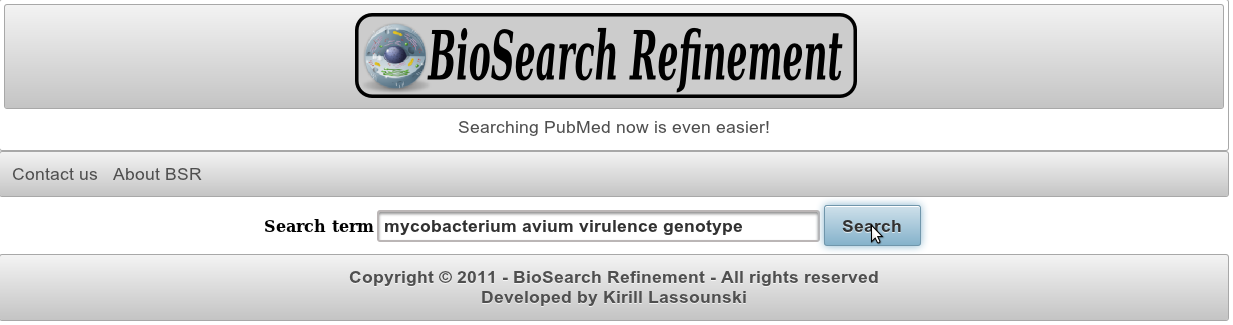
\includegraphics[scale=0.35]{imagens/telaInicial.png}
    \caption{Tela inicial do \emph{BioSearch Refinement} \label{fig:telaInicial}} 
\end{figure}

Na Figura \ref{fig:telaComBusca}, a aba foi aberta com o termo de busca solicitado e foram carregados os primeiros 20 artigos. Os artigos que são exibidos ficam guardados na memória (cacheados), se for feita a requisição para exibir outra página, e os artigos já exibidos ficam em \emph{cache} na sessão do navegador. Os artigos são exibidos em uma tabela similares à exibição do PubMed, informando o título, os autores, a revista na qual o trabalho foi publicado e o ano de publicação. Para visualizar informações complementares como o resumo do artigo, é necessário clicar na seta situada á esquerda para expandir um artigo.
\begin{figure}[h!]
    \center
    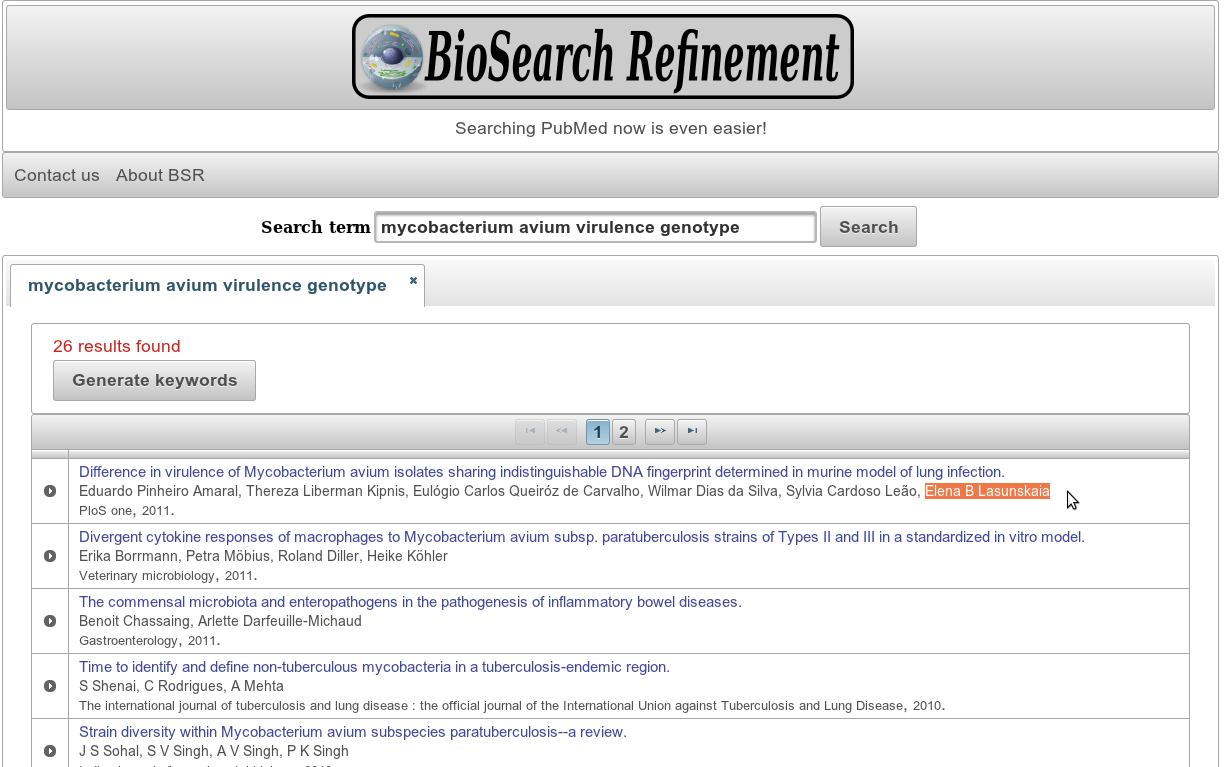
\includegraphics[scale=0.35]{imagens/telaComBusca.png}
    \caption{Tela após efetuar uma busca \label{fig:telaComBusca}} 
\end{figure}

Ao clicar no botão ''\emph{Generate keywords}'', o algoritmo \emph{Extraction Engine} é chamado para gerar as palavras-chave nos artigos que estão em \emph{cache}. Na Figura \ref{fig:palavrasChave} são mostradas as palavras-chave geradas para os artigos mostrados na figura anterior. Ao clicar em uma palavra-chave, uma nova aba será aberta. O título desta aba será o título da aba anterior concatenado com a palavra-chave selecionada, no exemplo da figura seria ''\emph{mycobacterium avium virulence genotype / mycobacterium avium subsp}''.

Existem dois tipos de abas no sistema, o primeiro se chama $LoadingTab$, esta aba representa o termo de busca inicial e implementa a paginação de artigos. A outra aba é a $OpenedTab$, gerada a partir de uma $LoadingTab$ e serve para mostrar os artigos refinados. Quando o usuário clica em uma palavra-chave, é aberta uma $OpenedTab$, e nesta aba as palavras-chave são recalculadas usando o \emph{Extraction Engine}. O processo de abertura de abas e processamento de palavras-chave é recursivo. 

As palavras-chave passam também por um processo de filtragem. Por exemplo, os termos que compõem o título da $LoadingTab$ da Figura \ref{fig:telaComBusca} (\emph{mycobacterium},\emph{avium},\emph{virulence},\emph{genotype}) são guardados em uma lista de \emph{stop words}. Se os termos da palavra-chave gerada pelo algoritmo \emph{Extraction Engine} estiverem na lista de \emph{stop words}, esta palavra-chave não será exibida, pois ela é irrelevante para o usuário. Ao abrir uma aba, a lista é incrementada com os termos da palavra-chave selecionada.

\begin{figure}[h!]
    \center
    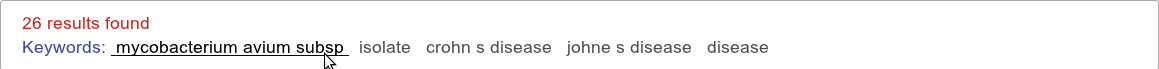
\includegraphics[scale=0.4]{imagens/palavrasChave.png}
    \caption{Palavras chave geradas pelo \emph{Extraction Engine} \label{fig:palavrasChave}} 
\end{figure}

\section{\emph{PubMed Dataset}}

Para avaliar o \emph{BioSearch Refinement} quanto à qualidade de suas predições e obter estatísticas importantes sobre os artigos do PubMed, é necessário um conjunto de programas que possibilitem a gestão destas informações. O \emph{PubMed Dataset} é uma API desenvolvida para a criação de conjuntos de dados teste com os artigos do PubMed, e também, serve como ponto de acesso ao PubMed no sistema \emph{BioSearch Refinement}. 

O objetivo principal do \emph{PubMed Dataset} é oferecer ao programador de um sistema de R.I. o acesso aos dados do PubMed através do E-Utils \cite{Eutils2010} e a capacidade de gravar e ler estes dados do disco através de um programa Java. Isto é feito através de conjuntos de dados \emph{datasets} que são salvos em disco através de serialização (uma técnica de persistência para objetos). Um conjunto de dados é constituído de artigos científicos que são recuperados do PubMed utilizando um termo de busca e uma configuração de \emph{download}.

\subsection{E-Utils}
O E-Utils é um \emph{Web Service} composto por um conjunto de programas que utilizam URL`s para fazer requisições e retornam dados em diversos formatos com HTML ou XML. Dentre estes programas, existem o E-Search, utilizado para fazer buscas e o E-Fetch para recuperar os dados. O arquivo estruturado XML do PubMed atende o padrão DTD do NLM Journal Archiving and Interchange, disponibilizado pelo NLM. O objetivo foi fornecer um formato comum que permitisse o intercâmbio de informação. Foram criados vários conjuntos de \emph{tags}, cada um com um propósito. Mas vale ressaltar que nem todos os artigos possuem todas as \emph{tags}, fato que deve cuidadosamente tratado com mecanismo de exceções. Dentre os elementos de um XML estão os seguintes elementos:

\begin{itemize}
    \item <PMID>: identificador único de um determinado artigo
    \item <Article>:  é o elemento raiz do documento, que contém todos os meta-dados e conteúdo do artigo.
    \item <ArticleTitle>:  contém o título de um artigo.
    \item <Abstract>:  descrição sumária do conteúdo de um artigo.
    \item <KeywordList>:  elemento que contém conjuntos de palavras-chave associadas com todo o documento e que podem ser usadas para fins de identificação e indexação. Estas palavras chave são atribuídas pelos autores do artigo.
    \item <MeshHeadingList>: lista de termos MeSH.
\end{itemize}
Estas informações são usadas pelo sistema \emph{BioSearch Refinement} para determinar as palavras-chave e exibir o conteúdo dos artigos.

\subsection{Funcionalidades}
A Figura \ref{fig:processoGeralPMD} apresenta o funcionamento geral da biblioteca PubMed Dataset. A partir de parâmetros de entradas especificados, a ferramenta se conecta à base de dados PubMed. O processo de obtenção do conjunto de dados envolve o processamento de documentos XML, que são retornados dos servidores do NCBI. Destes documentos são extraídos os dados requisitados pelo usuário através de uma configuração de \emph{download}.

\begin{figure}[h!]
    \center    
    \includegraphics[scale=0.5]{imagens/processoGeralPMD.pdf}
    \caption{Processo de obtenção de artigos do \emph{PubMed Dataset}\label{fig:processoGeralPMD}}
\end{figure}

Os parâmetros de entrada obrigatórios são:
\begin{itemize}
    \item o termo de busca que será utilizado para fazer uma query no banco de dados do
NCBI e que irá retornar um conjunto de artigos;
    \item número máximo de artigos a serem buscados para criar o conjunto de dados;
    \item os atributos que serão extraídos e usados para a criação das instâncias de um artigo.
Se um dos atributos não for encontrado em um artigo do XML, este artigo será
descartado. Como atributo de saída pode ser especificado qualquer elemento
presente no arquivo XML.
\end{itemize}

O arquivo de saída é um arquivo serializado no formato ( \emph{termo de busca\_número de artigos\_articles.ser}, ex: \emph{mycobacterium tuberculosis\_2754\_articles.ser}). Este arquivo pode ser desserializado a qualquer momento e os artigos contidos neste estarão disponíveis prontamente. Uma instância do diagrama de classes da biblioteca é apresentada na Figura \ref{fig:pubMedDatasetUML}.
\begin{figure}[h!]
    \center    
    \includegraphics[scale=0.24]{imagens/pubMedDatasetUML.pdf}
    \caption{Diagrama de classes UML do \emph{PubMed Dataset} \label{fig:pubMedDatasetUML}}
\end{figure}

O  $ArticleDownloader$ é a classe responsável por obter os artigos do banco de dados PubMed e é construída com uma configuração $DownloadConfiguration$. Se o número máximo de artigos solicitados for muito grande, o processo de obtenção de artigos é fracionado em partes para evitar time out por parte do servidor, isto é implementado no método $getDynaArticles()$ de $ArticleDownloader$. Primeiramente são obtidos os $PMID$’s através do E-Search e em seguida, utilizando estes, os artigos são recuperados e colocados em um DOM (\emph{Document Object Model}) utilizando o E-Fetch. O DOM é uma convenção para representar documentos XML e outros dentro de uma linguagem de programação. Em seguida, os elementos são percorridos e são
recuperados aqueles que foram selecionados pelo usuário no $DownloadConfiguration$.

\begin{itemize}
\item $DownloadConfiguration$ – é onde são definidas as configurações do download. São especificados os atributos que estarão presentes em cada artigo recuperado.
\begin{lstlisting}
DownloadConfiguration config = new DownloadConfiguration(ABSTRACT,AUTHOR,TITLE);
\end{lstlisting}

\item $DownloadParameter$ – É um enum no qual estão definidos os atributos que podem ser recuperados, estes atributos estão contidos em um $Map<String,Class>$ que define o nome e a classe de um atributo. Um título de artigo, por exemplo, possui $String = ''Title''$ e $Class = java.lang.String$, já uma lista de termos MeSH, possui $String = ''MeshTerms''$ e $Class = java.util.Set$, pois representa uma lista de termos.
\end{itemize}

Ao receber um $DownloadConfiguration$ o $ArticleDownloader$ pode efetuar a recuperação dos artigos através do método $getDynaArticles(termoDeBusca, maxHits)$ ou $getDynaArticles(termoDeBusca, primeiroArtigo, tamanhoDePagina)$. O primeiro método recebe um termo de busca, e o numero máximo de artigos que serão buscados no banco. O segundo método recupera uma fração de documentos, através dos dois últimos argumentos e pode ser usado para paginação. Ambos métodos retornam uma $List<DynaArticle>$ que possui as instâncias dos artigos que foram recuperados.

\begin{itemize}
\item $DynaArticle$ – Esta classe representa um artigo do PubMed. Possui uma
$Collection<Object>$ que serve para armazenar as palavras-chave geradas por um
algoritmo qualquer, e possui um $Map<String, ArticleAttribute>$ que serve para
guardar os atributos extraídos do PubMed. Um ponto importante é que esta classe por
possuir esta estrutura característica, permite que sejam criadas instâncias de artigos
dinamicamente, ou seja, com uma quantidade variável de atributos.

\item $ArticleAttribute$ – O atributo de um artigo é um dos fatores que permite a criação de
artigos dinâmicos. Esta classe possui nome do atributo, tipo do atributo e seu valor.

\end{itemize}
O $Dataset$ é quem vai encapsular os artigos e que será utilizado como unidade de persistência,
ou seja, será gravado em disco utilizando serialização. Mas esta classe nunca será utilizada
diretamente, pois possui um método abstrato chamado $generateKeyWords()$ que será
utilizado para o processo de geração de palavras-chave. Então, a utilização correta de um
$Dataset$ é se estendendo ele e implementando o método $generateKeyWords()$.

Como dito anteriormente, alguns artigos no PubMed podem não possuir determinados atributos, por isso o $ArticleDownloader$ possui uma variável booleana chamada $mandatoryAttributes$. Se o valor da variável for setado como \emph{true}, todos os atributos que foram passados na $DownloadConfiguration$ serão considerados obrigatórios, e os artigos que não possuírem algum destes atributos serão descartados.

Finalmente, a classe $DatasetSerializer$ é que faz a serialização e desserialização dos
$Dataset$`s. Na serialização, ela recebe o $Dataset$ a ser salvo em disco e um nome para o
arquivo que será salvo, geralmente um bom nome é o termo utilizado na criação do $Dataset$. A
este nome é acoplado o número de artigos existentes no $Dataset$ e a extensão “.ser” é
concatenada automaticamente. A desserialização é o processo inverso, no qual a partir do nome
de arquivo, o $Dataset$ é carregado para uma instancia.
É importante observar que quando o $Dataset$ é muito grande, pode ocorrer um erro de
\emph{java.lang.OutOfMemoryError: Java heap space}, pois a memória da máquina virtual Java
estoura e não consegue terminar a serialização ou o processo inverso. Para solucionar este
problema, a memória da maquina virtual deve ser aumentada, passando um parâmetro na linha
de comando:

\begin{lstlisting}
$ java -Xmx=256M seuProgramaQueEstouraAMemória
\end{lstlisting}

\section{\emph{Extraction Engine}}
O algoritmo \emph{Extraction Engine} foi desenvolvido como parte do sistema \emph{BioSearch Refinement} e é o componente do sistema que faz a extração das palavras-chave dos artigos e os organiza em tópicos mais abordados. A API de processamento de linguagem natural escolhida foi a \textbf{Alias-i Ling Pipe} que possui licença de uso gratuita para propósitos de pesquisa. Na recuperação e indexação dos artigos as palavras-chave jogam um papel integral, a extração de palavras-chave do corpo de um artigo tenta capturar a essência do assunto do mesmo, sem trabalhar com anotações humanas. A extração de palavras-chave é executada sobre os resumos dos artigos, pois a maioria dos artigos não disponibiliza o texto completo, mas apenas o resumo \cite{Hulth2003}.

A Figura \ref{fig:processoGeralEE} apresenta o esquema geral do algoritmo proposto para a obtenção das palavras-chave e a Figura \ref{fig:fluxoExecucaoEE} destaca um fluxo de execução para a obtenção de palavras-chave em um artigo. O algoritmo é dividido em vários passos, explicados a seguir. Para cada resumo:
\begin{figure}[h!]
    \center
    \includegraphics[scale=0.5]{imagens/processoGeralEE.pdf}
    \caption{Processo geral do algoritmo \emph{Extraction Engine} \label{fig:processoGeralEE}}
\end{figure}
\begin{figure}[h!]
    \center
    \includegraphics[scale=0.4]{imagens/fluxoExecucaoEE.pdf}
    \caption{Exemplo de obtenção de palavras-chave para um artigo \label{fig:fluxoExecucaoEE}}
\end{figure}
\begin{enumerate}
    \item \textbf{Divisão dos resumos em frases}: o texto de um resumo é composto por frases, um tokenizador trunca o texto em frases para utilizar na próxima etapa.

    \item \textbf{Rotulação ou POST (\emph{Part Of Speech Tagging})}: determina as classes gramaticais (\emph{tags}) de cada palavra na frase.

    \item \textbf{\emph{Noun Chunking}}: baseado no princípio de que os substantivos são os melhores descritores, o algoritmo seleciona termos compostos obrigatoriamente por substantivos. Para isto, foram definidos padrões sintáticos compostos por advérbios, adjetivos, numerais e alguns símbolos para conectar substantivos e formar termos mais descritivos.

    \item \textbf{Obtenção e seleção dos conceitos}: os conceitos servem para capturar a essência dos documentos e agrupar diversos \emph{noun chunks} similares em uma estrutura única. Um conceito é composto pelas palavras substantivas que compõem um \emph{chunk}, assim os termos \emph{green cells} e \emph{blue cells} fariam parte de um mesmo conceito \emph{cells}. São usados apenas os substantivos, pois o objetivo é generalizar o assunto sendo abordado no texto e agrupar assuntos semelhantes em um único conceito.

Para ilustrar a necessidade do uso de conceitos, observe os seguintes termos extraídos de um dos resumos: “\emph{other vegetable system}”, “\emph{the vegetable systems}” e “\emph{the vegetables}”. Se analisarmos as duas primeiras frases percebemos que elas tratam de um mesmo assunto “\emph{vegetable systems}”, porém a máquina irá tratar “\emph{system}”  e “\emph{systems}”  como duas palavras diferentes. Para contornar este tipo de discrepância é utilizado um algoritmo de normalização (\emph{stemming}). Usamos uma implementação do algoritmo de Porter \cite{Porter1980} fornecida pela API LingPipe, que permite remover sufixos de palavras em inglês.

Visto que as palavras são normalizadas, as frases “\emph{other vegetable system}” e “\emph{the vegetable systems}” são tratadas como sendo um mesmo conceito. Por outro lado, a terceira palavra só possui “\emph{vegetable}” como substantivo, o que acarreta na criação de um segundo conceito “\emph{vegetable}”.
\end{enumerate}



\subsection{Obtenção de conceitos}
O processo de conceitualização se divide em duas etapas. Na primeira, os conceitos são extraídos para cada artigo e são determinados os mais relevantes. Na segunda etapa, são selecionados os conceitos que abordam a maior quantidade de artigos diferentes, determinando assim os temas mais abordados pelos artigos.

\subsubsection{Conceitualização local}
O processo de conceitualização se inicia com a criação de uma estrutura de armazenamento de conceitos, mostrada na Figura \ref{fig:conceitualizacaoLocalUML} chamada $ArticleConcepts$, que irá conter os conceitos de um determinado artigo. Um conceito é composto por um ou mais termos e cada um destes termos possui uma frequência no texto e pode possuir variações no texto como por exemplo plurais. Por isso um $Concept$ é composto por diversas partes $ConceptPart$, onde cada parte possui:
\begin{itemize}
    \item Peso ($weight$): representa a interação das partes de outros conceitos com este conceito, um processo de cruzamento de informações explicado adiante.
    \item Raiz da parte ($partStem$): a raiz da palavra que compõe esta parte para a comparação com outras partes.
    \item Mapa de frequência de ocorrência ($partWords$): usado para contar as frequências das diferentes palavras que em algum momento fizeram parte deste conceito.
\end{itemize}

\begin{figure}[h!]
    \center
    \includegraphics[scale=0.35]{imagens/conceitualizacaoLocalUML.pdf}
    \caption{Diagrama de classes de conceitualização local \label{fig:conceitualizacaoLocalUML}}
\end{figure}

Ao se criar um conceito, automaticamente, são criadas suas $ConceptPart$ e este conceito é adicionado em $ArticleConcepts$. Termos iguais ou similares são agrupadas sob o mesmo conceito. Por exemplo: o conceito “\emph{other vegetable system}” possui três partes: “$other$”, “$vegetable$” e “$system$”.  Ao aparecer “\emph{the vegetable systems}”, os conceitos seriam integrados utilizando a estrutura a seguir. A comparação entre os termos é feita na raiz de suas partes substantivas.

Conceito: \emph{vegetable system}

Parte 1:$vegetable$, Raiz:$vegetable$, Mapa:$vegetabl$e (frequência: 2)

Parte 2:$system$, Raiz:$system$, Mapa:$system$ (frequência: 1), $systems$ (frequência: 1)

\subsubsection{Cruzamento de informações}
Para melhor descrever um artigo, é necessário avaliar cada conceito, valorizando os conceitos realmente relevantes e diminuindo o peso de conceitos pouco relevantes.

O processo de atribuição de peso de um conceito localmente é feito através um cruzamento de informação das partes de todos os conceitos similares a ele. Isso faz com que conceitos diferentes e com partes em comum recebam um peso maior, evidenciando ,assim, o grupo de conceitos que são mais abordados naquele artigo. Um conceito é similar a outro conceito, se estes possuem pelo menos uma parte em comum. A similaridade é calculada através da distância entre conceitos, e é a divisão do número de partes em comum pelo número de partes total do maior conceito.

A distância entre o $Conceito 1$ do exemplo anterior e o $Conceito 2$, a seguir, é calculado como:\newline
\textbf{
Conceito2: \emph{vegetable oil} \\
Partes em comum: 1 \\
Distância: ½ = 0.5}\\

O cruzamento de dois conceitos é feito para determinar o peso das partes similares, mostrado na Listagem \ref{lst:cruzamento}:
\lstset{caption={Cruzamento de dois conceitos},label=lst:cruzamento}
\begin{lstlisting}
    double weight = (fromPart.getPartFrequency() * distance);
    weight += toPart.getWeight();
    toPart.setWeight(weight);
\end{lstlisting}

Quanto maior a distância entre os conceitos, menor a influência de um no outro. O peso é atualizado para ambos os conceitos. Ao finalizar este processo, é feito o cálculo do peso dos conceitos utilizando-se do peso de suas partes, da frequência das partes e do número de partes que o conceito possui. O peso de um conceito é:

\(
\left(\sum_{partes}\medspace parte.frequencia + parte.peso\right) * \left(1 + fator\medspace de\medspace ajuste * num.\medspace de\medspace partes\right)
\)

Em primeiro lugar, é calculada a importância do conceito no texto do resumo. Para todas as partes de um conceito, é feito o somatório da sua frequência no texto e da sua interação com outros conceitos similares (peso do conceito). Este valor é então multiplicado pelo segundo parenteses da equação, onde é dada prioridade aos conceitos que possuem mais partes. Conceitos com mais partes são mais representativos, logo mais importantes. Além de aumentar a representatividade dos conceitos é feito o balanceamento entre a pequena quantidade de conceitos com muitas partes e pouca frequência e de conceitos com poucas partes e frequência alta. O fator de ajuste foi considerado 0.05 para que a cada parte que o conceito possui, ele receba um aumento no seu peso de 5\%, logo em um conceito de 4 partes este aumento é de 20\%. O valor do fator de ajuste foi determinado empiricamente.

Ao fim do processo, conceitos de apenas uma palavra e com menos de 4 letras são removidos, considerados pouco representativos.
Os conceitos com o maior peso são aqueles que foram mais referenciados no resumo, logo, são os melhores descritores. Cada conceito obtido pelo algoritmo é linearmente mapeado em uma predição de palavra-chave do artigo. Este processo é repetido para todos os resumos.

\subsubsection{Conceitualização global}

O processo de obtenção de conceitos é realizado em cada resumo de artigo. O conceito que referencia o maior número de artigos distintos tem maior importância, pois ele trata de um assunto comum, ou seja, é mais abordado em todos os artigos e passa a formar parte das palavras-chave globais. As palavras-chave globais formam o melhor conjunto de descritores para todos os artigos recuperados em uma consulta.

Cada conjunto de conceitos local é ordenado pelo peso decrescentemente, e deste conjunto apenas uma parte é selecionada para a conceitualização global. O principal motivo deste corte é a exclusão de conceitos pouco descritivos ou muito gerais que possuem pontuação relativamente baixa, e em segundo lugar a melhora da performance do sistema através da diminuição de conceitos a serem processados na fase global.

Resumos com maior quantidade de texto possuem mais palavras-chave do que resumos com algumas linhas, por isso a quantidade de conceitos selecionada é uma porcentagem do total de conceitos extraídos de um resumo. Foi verificado através de testes que os melhores resultados eram obtidos com a seleção de 35\% dos conceitos, assim eliminando 65\%.

No processo de globalização, os conceitos locais passam por uma verificação de integração, que permite que um mesmo conceito extraído de vários artigos seja unificado em um só. A unificação de conceitos implica na atualização da frequência desse conceito. Após a análise de todos os conceitos de todos os artigos, é feita a ordenação decrescente, seguindo os critérios: frequência (número de artigos que o referenciam) e peso do conceito. Os conceitos que possuem o maior número de artigos sendo referenciados, são os conceitos com maior abrangência, logo são considerados as melhores palavras-chave para sumarização.

Na \emph{interface} são exibidas as cinco melhores predições, mas algumas podem ser descartadas pelo algoritmo por serem consideradas como \emph{stop words}.

\subsection{Implementação}
Na Figura \ref{fig:conceitualizacaoUML} está representado o diagrama de classes do \emph{Extraction Engine}.
A classe que faz o processamento dos artigos é a $KeyWordProcessor$, ela também dá acesso aos conceitos mais referenciados através de um $Iterator<Concept>$ pelo método $getConceptIt()$. O método $processArticles$ recebe os artigos a serem processados e chama $conceptualize$. Este método irá percorrer todos os artigos, recuperar os resumos de cada um deles e tokenizá-los em frases usando o $SentenceSplitter$.

\begin{figure}[h!]
    \center
    \includegraphics[scale=0.25]{imagens/conceitualizacaoUML.pdf}
    \caption{Diagrama de classes de conceitualização\label{fig:conceitualizacaoUML}}
\end{figure}

As frases são passadas para o $MedLineSentenceChunker$ que determina os $TaggedChunk$`s de cada frase. Estes \emph{chunks} são usados na conceitualização local explicada anteriormente para determinar os conceitos mais relevantes de um artigo.

Os conceitos obtidos localmente são guardados no $GlobalConceptHolder$ através do método $insertConcept$. A cada conceito que é inserido, é feita uma busca para determinar se um conceito parecido conceitualmente já existe. A comparação de dois conceitos é feita através de uma chave, que é composta pelas raízes das partes de um conceito. Se dois conceitos são similares, a lista de PMID`s deste conceito é incrementada como também a frequência de ocorrência de suas partes.

Após todos os conceitos serem inseridos no $GlobalConceptHolder$, é chamado o método $sortConcepts$ para que os conceitos sejam ordenados segundo o seu número de PMID`s e depois por frequência de ocorrência. Nesta etapa o \emph{BioSearch Refinement} já pode obter o $Iterator<Concept>$ para navegar pelos conceitos mais referenciados e selecionar as palavras-chave.
